%Laborationsrapport

\documentclass[a4paper,12pt,fleqn]{article}
\usepackage{fixltx2e}
\usepackage[utf8]{inputenc}
\usepackage{graphicx}
\usepackage{sidecap}
\usepackage{fancyhdr}
\usepackage{amssymb,amsmath}
\usepackage[swedish]{babel}
\usepackage[margin=1.5in]{geometry}
\usepackage{abstract}
\usepackage[parfill]{parskip}
\usepackage{tocloft}
\usepackage{adjustbox}
\usepackage{textcomp}
\usepackage[T1]{fontenc}
\usepackage{listings}
\usepackage{xcolor,colortbl}
\usepackage{hyperref}
\usepackage{amsmath}

%----------------------------------------------------------------
%C-kod formatering

\definecolor{listinggray}{gray}{0.9}
\definecolor{lbcolor}{rgb}{0.9,0.9,0.9}
\lstset{
backgroundcolor=\color{lbcolor},
    tabsize=4,    
%   rulecolor=,
    language=[GNU]C++,
        basicstyle=\scriptsize,
        upquote=true,
        aboveskip={1.5\baselineskip},
        columns=fixed,
        showstringspaces=false,
        extendedchars=false,
        breaklines=true,
        prebreak = \raisebox{0ex}[0ex][0ex]{\ensuremath{\hookleftarrow}},
        frame=single,
        numbers=left,
        showtabs=false,
        showspaces=false,
        showstringspaces=false,
        identifierstyle=\ttfamily,
        keywordstyle=\color[rgb]{0,0,1},
        commentstyle=\color[rgb]{0.026,0.112,0.095},
        stringstyle=\color[rgb]{0.627,0.126,0.941},
        numberstyle=\color[rgb]{0.205, 0.142, 0.73},
%        \lstdefinestyle{C++}{language=C++,style=numbers}’.
}
\lstset{
    backgroundcolor=\color{lbcolor},
    tabsize=4,
  language=C++,
  captionpos=b,
  tabsize=3,
  frame=lines,
  numbers=left,
  numberstyle=\tiny,
  numbersep=5pt,
  breaklines=true,
  showstringspaces=false,
  basicstyle=\footnotesize,
%  identifierstyle=\color{magenta},
  keywordstyle=\color[rgb]{0,0,1},
  commentstyle=\color{Darkgreen},
  stringstyle=\color{red}
  }
  %-----------------------------------------------------------------
  %marginaler

  \renewcommand{\abstractnamefont}{\normalfont\normalsize\bfseries}
  \renewcommand{\abstracttextfont}{\normalfont\small}
  \renewcommand{\headrulewidth}{0pt}
  \renewcommand{\cftsecleader}{\cftdotfill{\cftdotsep}} 
  \setlength{\absleftindent}{0pt}
  \setlength{\absrightindent}{0pt}
  \setlength{\headheight}{15pt}

  \addtolength{\oddsidemargin}{-.5in}
  	\addtolength{\evensidemargin}{-.5in}
  	\addtolength{\textwidth}{1in}


  %-----------------------------------------------------------------
  %header and footer

  \pagestyle{fancy}
  \lhead{
  	\begin{picture}(0,0)
  		\put(5,0){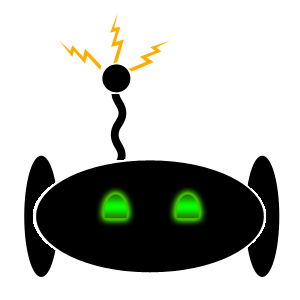
\includegraphics{logotyp.png}}
  	\end{picture}}
	
  \fancyhead[C]{\small{Mapmaster2001}}
  \fancyhead[R]{\small \today}
  \fancyfoot[L]{\small{TSEA56 \\ LIPS Kappa}}
  \fancyfoot[C]{\small{\thepage}}
  \fancyfoot[R]{\small{Projektgrupp 8 \\ mapmaster2001@cyd.liu.se}}

  %-----------------------------------------------------------------

%-------------------------------------------------------------------
%Första sidan

\begin{document}
	\pagestyle{fancy}
\pagenumbering{roman}
	\vspace*{\fill}
		\begingroup
			\begin{center}
				\huge{\textbf{Sensorers applikation för kartritande robot}}
				\\
				\vspace{10pt}
				\normalsize
				Erik Ekelund och David Habrman
				\\
				Kandidatprojekt Y - Grupp 8 - VT2014
				\\
				Version 1.0
				\end{center}
		\endgroup
	\vspace*{\fill}
	
	\begin{center} %Börjar centrering 
		Status
		\\
		\vspace{3pt} %Whitespace 3 pts
	    \begin{tabular}{| p{3cm} | p{3cm} | p{3cm} |} %tabell, 4 horizontella |, 3 cm emellan dem.
	    \hline %översta horizontella linjen.
	    Granskad & - & \today \\ \hline % & -tecken för att "gå till nästa ruta" 
		Godkänd & - & - \\ \hline % avslutas med \\ och \hline.

	    \end{tabular}
	\end{center}
	\vspace{2cm}
	\newpage
%-----------------------------------------------------------------
%Projektidentitet
	
	\vspace*{\fill}
		\begingroup
			\begin{center}
				\LARGE{\textbf{PROJEKTIDENTITET}}
				\\
				\footnotesize
				Grupp 8, 2014/VT, MapMaster2001
				\\
				Linköpings tekniska högskola, ISY
				\\
				\vspace{1cm}
	  \begin{tabular}{| p{3cm} | p{4.3cm} | p{2.4cm} | p{3.8cm} |}
	    \hline
		\textbf{Namn} & \textbf{Ansvar} & \textbf{Telefon} & \textbf{E-post} \\ \hline
	    Jens Edhammer & Dokumentanvsvarig (DOK) & 076-030 67 80 & jened502@student.liu.se \\ \hline
		Erik Ekelund & Designansvarig (DES) & 073-682 43 06 & eriek984@student.liu.se \\ \hline
		David Habrman &  & 976-017 71 15 & davha227@student.liu.se \\ \hline 
		Tobias Grundström & Testansvarig (TES) & 073-830 44 45 & tobgr602@student.liu.se \\ \hline 
		Hans-Filip Elo &   & 073-385 22 32 & hanel742@student.liu.se \\ \hline 
		Niklas Ericson & Projektledare (PL) & 073-052 27 05 & niker917@student.liu.se \\ \hline
	    \end{tabular}
		
		\vspace{1cm}
		\textbf{E-postlista för hela gruppen:} mapmaster2001@cyd.liu.se
		\\[0.5cm]
		
		\textbf{Kund}: Mattias Krysander, Linköpings Universitet, 581 83  LINKÖPING, \\
		013-28 21 98, matkr@isy.liu.se \\
		\textbf{Kontaktperson hos kund}: Mattias Krysander, 013-28 21 98,matkr@isy.liu.se 
		\\
		\textbf{Kursansvarig}: Tomas Svensson, 3B:528,013 28 21 59,tomass@isy.liu.se
		\\[0.5cm]
		\textbf{Handledare}: Peter Johansson, 013-28 1345 peter.a.johansson@liu.se

				\end{center}
		\endgroup
	\vspace*{\fill}
\newpage

%-----------------------------------------------------------------
%Innehållsföreteckning

\addto\captionsswedish{\renewcommand{\contentsname}{Innehållsförteckning}}

\tableofcontents
\thispagestyle{fancy}
\newpage

\pagenumbering{arabic}
%-----------------------------------------------------------------
%Översikt
\section{Inledning}

Disposition: 
\\
1. Inledning 
\\
2. Problemformulering (frågeställningar som rapporten ska behandla) 
\\
3. Kunskapsbas (litteratur, datablad, dokumentation, etc.) 
\\
4. Fördjupningstext (modeller, beräkningar, analyser och eventuella experiment) 
\\
5. Resultat och slutsatser 
%-----------------------------------------------------------------

Syftet med denna rapport är att belysa och undersöka olika optiska-, ljud- och accelerationssensorers användbarhet för autonom navigering.
Rapporten kommer att belysa olika fördelar med de olika teknikerna samt vilka sensortyper som är att föredra i olika situationer.
Rapporten kommer även att granska hur sensorerna presterar, hur känsliga de är för störningar samt om det finns variationer av teknikerna.
Sensorerna som kommer undersökas är av de typer som finns tillgängliga på Linköpings Universitet vid institutionen för systemteknik för studenter som i kursen Elektronikprojekt.


%-----------------------------------------------------------------
\section{Problemformulering}
Autonoma robotar blir allt vanligare och påträffas i allt från konstruktionsrobotar i industrimiljö till självgående gräsklippare för privatpersoner.
Vid konstruktion av en autonom robot finns det i nuläget  en uppsjö av tekniker att använda för att navigera. Det vi söker att besvara är hur dessa olika tekniker fungerar samt hur de kan tillämpas för att på ett effektivt sätt hjälpa självgående robot att utföra sitt uppdrag.
Vidare söks även nackdelar med de olika teknikerna, hur dessa kan undvikas och vilka styrkor de olika teknikerna har gentemot varandra.

Frågorna som rapporten kommer att behandla är:
\begin{itemize}

\item Hur fungerar en optisk sensor? 
\item Hur noggrann är en optisk sensor?
\item Hur känslig är den för störningar?
\item Vad är nackdelarna respektive fördelarna med en optisk sensor?

\item Hur fungerar Time of flight sensorer?
\item Vilka typer finns det?
\item Vilka fördelar respektive nackdelar har de?

\item Hur fungerar en accelerometer? 
\item Hur klarar en accelerometer störningar?

\item Hur fungerar en RFID-läsare?
\item Vilka svagheter och styrkor har tekniken?

\item Hur kan sensorerna användas för att navigera?
\item Vilka sensorer passar sig bäst för en labyrintnavigerande och kartritande robot?
\end{itemize}

%-----------------------------------------------------------------
\section{Fördjupningstext}
\subsection{Avståndsmätare}
En optisk sensor är ett typ av instrument som används för att med hjälp av ljus mäta avstånd till en yta.

Sensorn som beskrivs nedan är av single-baseline optiksensor, vilket betyder att den opererar med endast ett sändar- och mottagarpar, och bedömer avstånd med hjälp av en typ av triangulering.
En typisk single-baseline optisk sensor kräver fyra grundkomponenter för att fungera.
En ljuskälla i form av t.ex. en laser, en lins för att fokusera det reflekterade ljuset på 
en optisk sensor, samt en yta att reflektera ljuset mot, dvs ytan som avståndet skall mätas till.

Ljuskällan riktas rakt mot den yta som avståndet ska mätas till och en ljuspuls avfyras. Ojämnheter i ytan gör att ljuspulsen reflekteras åt flera håll. Några av dessa ljusreflektioner kommer med största sannolikhet att studsa tillbaka mot sändaren.
Strax under ljuskällan sitter en svagt vinklad sensor som tar emot den reflekterade ljuspulsen.  Vart på sensorn som det reflekterade ljusets högsta koncentration uppmäts bestämmer medhjälp av trigonometri på vilket avstånd som avståndsmätaren uppfattar att reflektorn ligger.


För att beräkna avståndet till reflektionskällan krävs kunskap om tre saker.
Det lodräta avståndet mellan ljuskällan, även kallat måttstocken, vinklarna i de två trianglar som ljuskälla, lins, sensor och måttstockens startpunkt bildar. Slutligen krävs positionen på sensorn där det reflekterade ljustets intensitet är störst. Sensorn placerad så att linsens fokalpunkt, det lodräta avstånd till den punkt där parallella ljusstrålar sammanfaller i ett maximum, ligger precis i djup med sensorn. Denna placering är logisk då detta får de infallande ljustrålarna att sammanfalla perfekt då de når sensorytan, vilket i sin tur ger högst intensitet.

\subsection{Triangulering}
Triangulering är en avståndsbetämingsmetod som använder kända vinklar och simpel geometri för att bestämma det lodräta avståndet till ett föremål.
Om det horisontella avståndet, \begin{math}\delta\end{math} är känt så fås det lodräta avståndet till punkten P av:
\begin{equation}
\label{eq:angle}
\frac{P}{\delta}=tan(\beta)
\end{equation}
Denna ekvation kan vara missledande då den ger intrycket av att det inte finns maximal och minimal uppmätbar distans vilket tyvärr är fallet för optiska triangulationssensorer.
Det finns nämligen ett antal faktorer som tillsammans bestämmer sensorns egenskaper.

I fallet med optisk sensor bestäms vinkeln \begin{math}\beta\end{math} med hjälp av de kända avstånden D och f. D ges av den optiska sensorn medans f är känt som linsens fokallängd. Om ett infallande ljusknippe infaller på sensorn kan \begin{math}\beta\end{math} bestämmas och därmed P, men om  infallsvinkeln blir tillräckligt stor så kommer det reflekterade ljusknippet att missa sensorn vilket kommer leda till att vinkeln inte kan bestämmas.

Sensorns effektiva mätområde är alltså beroende på sensorns bredd, linsens fokallängd och avståndet mellan sensor och sändare.
En ökad sensorstorlek ger ett större omfång medans ett minskat avstånd mellan sensor och sändare förskjuter omfånget så att sensorns maximala räckvidd ökar. Att minska avståndet medför dock att systemet blir mindre och mindre linjärt, dvs att ett inkrement i P inte linjärt ökar vinkelutslaget.

\subsection{Time-Of-Flight sensorer}
En typ av sensor som används för avståndsbestämning är typen time-of-flight även känt som TOF sensorn. Dessa typer av sensorer bestämmer avståndet till ett objekt genom att betrakta en reflekterad vågs egenskaper. 
En våg skickas ut från en emitter mot ett objekt. Vågen som sedan studsar tillbaka uppfattas av en mottagare som är gjord för att uppfatta vågor av samma typ som emittern skickar. Vågtypens hastighet i det aktuella mediet v, tillsammans med tidsfördröjnignen T för ekot samt vågens fasskifte används för att bestämma avståndet.



\subsection{Variationer av TOF-sensorer}

\subsubsection{Pulse modulation}
Den finns flera olika typer av TOF-sensorer som inriktar sig på att mäta andra vågengenskaper och en av dem är pulsmodulation.
TOF-typen pulse modulation skickar iväg en puls med en känd längd \begin{math}T_{0}\end{math}. Tiden från start på den utgående pulsen tills dess att mottagaren registrerar en reflekterad våg \begin{math}T_{D}\end{math} uppmäts och används tillsammans med vågtypens hastighet i mediet för att beräkna avståndet till föremålet som orsakat ekot. Formeln för detta ses i ekvation \ref{eq:distance}
\begin{equation}
\label{eq:distance}
d = \frac{1}{2}*v_{medium} \cdot T_D
\end{equation}

\subsubsection{Sinusmodulation}
TOF-tekniken sine wave modulation bestämmer avstånd med hjälp av att mäta fasskiftet \begin{math}\delta\phi\end{math} mellan sinusmodulerad utsignal och dess reflektion. Avståndet d, beräknas med hjälp av ekvation \ref{eq:distance2} där \begin{math}f_1\end{math} är modulationsfrekvensen. 
%http://www.srttu.edu/Teacher_Article/178.pdf
\begin{equation}
\label{eq:distance2}
\delta\phi = 2\pi \cdot \frac{2d}{v_{medie}}
\end{equation}


\subsubsection{Ljud- vs ljusvågor}
Då alla typer av vågor fungerar för att använda TOF-sensorer är det intressant att betrakta fördelarna och nackdelarna mellan att använda elektromagnetiska vågor och ljudvågor.
Då en elektromagnetisk våg rör sig otroligt snabbt kommer en extremt snabb intern klocka krävas för att uppskatta små förändringar i avståndet. Om mottagaren som minst kan uppmäta en tidsdifferens, \begin{math}\delta t\end{math} , på en mikrosekund ges den minimala avståndsskilnaden som kan uppskattas av ekvation \ref{eq:diff}.

\begin{equation}
\label{eq:diff}
\begin{split}
\delta d & = v_{ljus}\cdot\delta t \\
& = 300 m
\end{split}
\end{equation}

Om sensorn istället använder ljud för att mäta avstånd men arbetar med samma minimumtid fås ett \begin{math}\delta d\end{math} enligt ekvation \ref{eq:diff2}.
Ljud ger alltså en flera magnituder bättre upplösning.
\begin{equation}
\label{eq:diff2}
\begin{split}
\delta d & = v_{ljud}\cdot\delta t \\
& = 0.34 mm
\end{split}
\end{equation}

Då ljud är långsammare kommer det dock att ta längre tid innan sensorn uppfattar en reflekterad våg, vilket kan innebära problem för system som behöver reagera extremt snabbt på förändringar. Vill man ha ett snabbt system bör man alltså överväga en ljussensor men detta medför i sin tur höga krav på sampling för att uppnå acceptabel noggrannhet.

En annan fördel med ljus är att det är lättare att rikta än ljud. Då ljud sänds ut finns det risk att ljudvågen studsar på någon oönskad yta vilket ger en felaktig uppskattning.
Ljus kan riktas mycket mer precis med tekniker som t.ex laser vilket till stor del eliminerar dessa typer av fel.



\subsection{Ultraljudsavståndsmätare}
Ultraljudssensorer använder sig av samma princip som fladdermöss och radar som uppsakattar avståndet till ett objekt genom att tolka dess eko från ljudsvågor. Med en högtalare genererar ultraljudssensorer högfrekvent ljud som studsar mot olika objekt. Ekot mottas och detekteras sedan av en ljudsensor. Ultraljudssensorn beräknar sedan tiden mellan utskick av ljud till mottagning av ekot. Eftersom ljudhastigheten i olika medium är känd kan avståndet till ett objekt beräknas med enkel matematik. En ultraljudssensor använder sig ofta av en transducer som omvandlar elektrisk energi till högfrekventa ultraljudsvågor och en för att omvandla ljudvågor till elektrisk energi som kan mätas.

En transducer är en komponent som konverterar energi till ultraljudsvågor. En hundvissla är ett exempel på en transducer, den omvandlar mekanisk energi från lufttryck till ljudvågor men de som används i avståndssensorer är betydligt mer komplicerade. Dessa konverterar elektrisk energi till ultraljudsvågor och består av piezoelektriska kristaller. Piezoelektriska kristaller ändrar storlek när man tillsätter en spänning. Genom att applicera en växelpänning över kristallerna kan man få dem att oscillera i väldigt höga frekvenser och på så sätt skapa högfrekventa ljudvågor. Efterson dessa kristaller genererar en spänning när en kraft verkar på dem så kan de kristaller som används för att skapa ljudvågorna även användas för att ta emot ekot.
\footnote{http://sv.wikipedia.org/wiki/Piezoelektricitet}

Fördelar med avståndsmätare som använder sig av ultraljud är att de inte är känsliga för färg, och transparens på det objekt man vill mäta avståndet till. De är heller inte känsliga för miljön, t.ex. dimma, ljusförhållanden, damm och smuts.

En nackdel med ultraljudmätaren vi har tillgång till (Devantech SRF04 Utrasonic Range Finder) är att den mäter avståndet till det närmaste objektet i en kon. Om man vill mäta avståndet till en vägg rakt framför roboten kan det, om konen är för bred, hända att roboten istället mäter avståndet till väggen på sidan av roboten. En annan nackdel är att den inte kan mäta avståndet till ljuddämpande material.
\footnote{https://docs.isy.liu.se/twiki/pub/VanHeden/DataSheets/srf04.pdf}


\subsection{Gyroskop}
Ett gyroskop är en sensor som används för att mäta vinkelhastigheten. För att göra detta använder man sig av corioliseffekten. Därför måste vi, för att förstå hur ett gyro fungerar, alltså först förstå corioliseffekten. Corioliseffekten beskriver hur rörliga objekts rörelseriktningar förändras när de betraktas av en observatör i en roterande referensram. Corioliskraften är den kraft som hör samman med effekten och är proportionell på rotationshastigheten. Kraften är liten men påverkar stora luftmassor då de rör sig över stora avstånd och långa tidsperioder. T.ex. så är det corioloskraften som får orkaner att rotera. Ett gyro är känsligt för corioliskraften och använder sig av den för att mäta vinkelhastighet.

Figur \ref{fig:jord} visar ett exempel på corioliseffekten. Vi tänker oss att den röda pricken är ett objekt i rörelse och den gröna pricken är en observatör som står stilla på den roterande jorden. Jorden blir då den roterande referensramen. Objektet rör sig söder ut sett från en inertialram, säg rymden. Observatören, som befinner sig öster om objektet, rör sig längsmed jorden och uppfattar därför inte objektets bana på samma sätt. Han ser en bana som är krökt åt väster.
\footnote{http://sv.wikipedia.org/wiki/Corioliseffekten}


\begin{figure}[h]
\label{fig:jord}
\caption{}
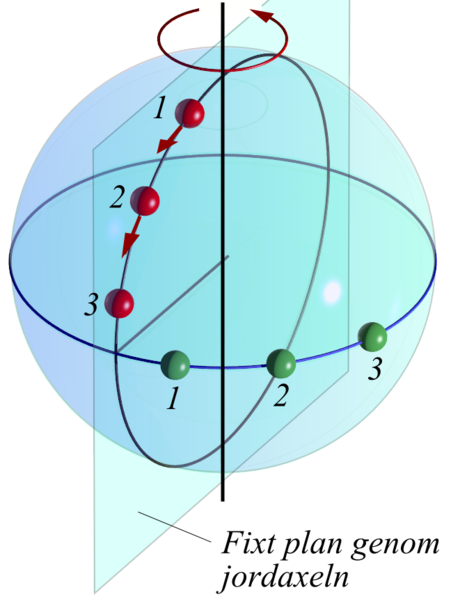
\includegraphics[width=0.3\textwidth]
{Coriolisjord.png}
\end{figure}


Namnet  gyroskop kommer från det grekiska ordet “skopeein” som betyder “att se” och det grekiska ordet “gyros” som betyder “rotation”. Det var Léon Foucault som kombinerade orden under han experimenterade med att mäta jordens rotation.

I figur \ref{fig:gyro} nedan visas ett simpelt gyroskop. Det byggs upp av ett snurrande hjul eller skiva på en axel som kan röra sig fritt. Eftersom att axeln inte vill byta riktning kan detta redskap användas för att bl.a. stabilisera fordon. Dessa gyroskop är dock stora och är inte helt friktionsfria. Utvecklingen gick vidare och man tog fram gyroskop som utnyttjade vibrationer.

\begin{figure}[h]
\label{fig:gyro}
\caption{}
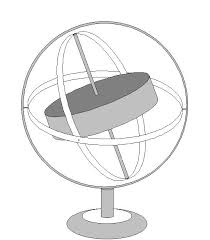
\includegraphics[width=0.3\textwidth]
{gyro.jpeg}
\end{figure}

De gyroskop som används mest idag, i t.ex. mobiler, är MEMS-gyroskop. MEMS kombinerar elektroniska och mekaniska system på micronivå. MEMS-systemen som används i gyroskop består av ett element som börjar vibrera när gyrot rör sig. Styrkan på dessa vibrationer kan mästas och för att göra det använder man sig av kapacitans.

MEMS-gyroskop tar idén från gyroskopen ovan men använder sig av MEMS istället för ett balanserat hjul på en axel. MEMS gyroskop använder sig av corioliseffekten för att mäta vinkelhastigheten. Figur \ref{fig:corilois} visar hur en massa påverkas av effekten.
\begin{figure}[h]
\label{fig:coriolis}
\caption{}
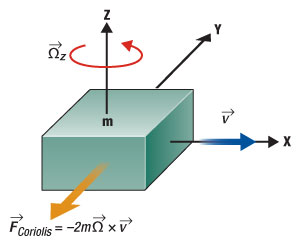
\includegraphics[width=0.3\textwidth]
{coriolis.png}
\end{figure}


När massan m rör sig med hastigheten v längs x-axeln och med vinkelhastihteten (ohmtecknet) runt z-axeln så uppstår en corioliskraft (den gula pilen). Den fysiska förflyttningen som orsakas av corioliskraften kan läsas av med den kapacitiva MEMS-sensorn. De flesta MEMS-gyroskopen använder sig av två massor som oscillerar konstant i motsatta riktningar, detta illustreras i figur \ref{fig:angular}. När man roterar massorna verkar då även corioliskraften åt olika håll vilket resulterar i att kapacitansen ändrar sig. Skillnaden i kapacitans är proportionell på vinkelhastigheten och konverteras sedan till en analog eller digital utsignal.

\begin{figure}[h]
\label{fig:angular}
\caption{}
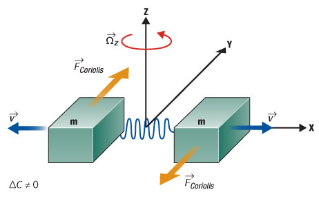
\includegraphics[width=0.3\textwidth]
{angularv.png}
\end{figure}

När man applicerar en linjär acceleration på massorna så rör de sig i samma riktning och det blir därför ingen ändring i kapacitans. Gyroskopet känner alltså inte av denna acceleration vilket gör att MEMS-gyroskop inte är känsliga för linjär acceleration så som stötar och vibration. De mäter alltså bara rotation.
\footnote{http://electroiq.com/blog/2010/11/introduction-to-mems-gyroscopes/}


MEMS-gyroskop mäter vinkelhastighet och har fler applikationsområden. Dessa används t.ex. i bildstabilisatorer. Gyrot detekterar då kamerans rotation och kameran kan då kompensera för rotationen och ge en skarp bild. De används också i mobiler, t.ex. för att rotera bilden, bilar, för att utlösa airbags, flygplan o.s.v.

MEMS-gyroskops mätområde anges i dps, grader per sekund (degrees per second). Den talar alltså om hur snabbt gyrot kan röra sig varje sekund och fortfarande ge en korrekt utsignal. Gyroskopen har också en form av upplösning som ofta anges i mV/dps, alltså hur mycket spänning som läggs på utsignalen per dps.

\subsubsection{Fördelar och nackdelar}
MEMS-gyroskop är billiga att masstillverka, de är små och de är strömsnåla. Detta har lett till att de blivit väldigt populära och används i mängder av handhållen teknik.
Gyron kan användas för att bestämma vinkel, men detta kräver en integrering eller en summering över tiden. Detta kan leda till problem i vissa system då samplat data behöver lagras.
\footnote{https://docs.isy.liu.se/twiki/pub/VanHeden/DataSheets/MLX90609_datasheet.pdf}

\subsection{RFID}
RFID står för radio-frequency identification och används för att läsa information från objekt, så kallade taggar, trådlöst via radiovågor. RFID kan delas in i flera olika grupper. Den billigaste, och den vi har tillgång till i kursen, kallas passiv RFID. I den passiva tekniken består taggarna av ett unikt nummer som endast kan läsas inom korta avstånd, ofta någon decimeter. Detta nummer kan sedan användas för att peka ut en plats i en databas med ytterligare information om taggen. Taggen består av ett microchip med en antenn men ingen egen strömkälla. Även läsaren har en antenn som skickar ut radiofrekvent energi. Energin från läsaren kan sedan tas upp av taggens antenn och konverteras till elektricitet. Microchippet i taggen får ström, kan modulera vågorna och skickar tillbaka dem till läsaren. Läsaren tar emot vågorna och omvandlar dem till digitalt data som motsvarar taggens nummer.
\footnote{https://docs.isy.liu.se/twiki/pub/VanHeden/DataSheets/rfid-reader-v21.pdf}

Aktiva RFID-raggar har, till skillnad från passiva taggar, sina egna strömkällor och även en sändare.

RFID kan användas på många sätt, t.ex. kan man sätta en tagg på en matvara, när en RFID-läsare läser av taggen kan den hämta information om varan i en databas. Taggarna fyller då ungefär samma funktion som streckkoder och man får då ett system med tre delar. Del ett är taggar, del två en läsare och del tre en databas med information om varje tagg. Taggarna kan göras väldigt små och tekniken används i bl.a. passerkort.

\subsubsection{Fördelar och nackdelar}
Tack vare den egna strömkällan i aktiv RFID kan läsavståndet göras betydligt mycket större än för den passiva tekniken. Aktiva taggar är dock större, dyrare och kräver mer underhåll än passiva taggar. Passiv RFID reflekterar dock bara en modulerad signal från läsaren. Det är därför läsavståndet inte är så långt.
\footnote{http://electronics.howstuffworks.com/gadgets/high-tech-gadgets/rfid3.htm}


\section{Resultat och slutsatser}

I våra undersökningar kom vi fram till att avståndsmätning med ultraljud inte är något för oss. Ultraljudsmätaren mäter avståndet i en kon och detekterar anståndet till närmaste objektet innanför konen. Detta kan göra att roboten detekterar avståndet till en sidovägg när man egentligen vill mäta avståndet till en vägg rakt framför roboten.

Gyrosop kommer att vara väldigt användbart för oss. Det kommer att underlätta beräkningar av robotens svängar. Då gyrot inte är känsligt för linjära accelerationer utan bara för rotationer så blir den användbar vid beräkningar av robotens svängar och körriktning.

Eftersom att en brandhärd kommer att representeras av en RFID-tagg i tävlingen så är RFID-läsaren en komponent som självklart kommer att vara en del av vår robot. Det finns ingen möjlighet för oss att välja mellan aktiv eller passiv teknik då de komponenter vi har tillgång till endast är för passiv RFID. Man skulle kunna tänka sig att använda aktiv för kunna detektera taggen från längre avstånd men då förändras tävlingsförutsättningarna och det skulle alltså bli en helt annorlunda tävling.

\section{Källförteckning}

Piezoelektricitet, wikipedia.org. Hämtad \today:
http://sv.wikipedia.org/wiki/Piezoelektricitet

Datablad för SRF04, Institutionen för systemteknik vid Linköpings Universitet. Hämtad \today:
https://docs.isy.liu.se/twiki/pub/VanHeden/DataSheets/srf04.pdf

Corioliseffekten, wikipedia.org. Hämtad \today:
http://sv.wikipedia.org/wiki/Corioliseffekten

Introduction to MEMS gyroscopes, electroiq.com. Hämtad \today:
http://electroiq.com/blog/2010/11/introduction-to-mems-gyroscopes/

Datablad för MLX90609, Institutionen för systemteknik vid Linköpings Universitet. Hämtad \today: https://docs.isy.liu.se/twiki/pub/VanHeden/DataSheets/MLX90609_datasheet.pdf

Datablad för Parallax-Reader, Institutionen för systemteknik vid Linköpings Universitet. Hämtad \today:
https://docs.isy.liu.se/twiki/pub/VanHeden/DataSheets/rfid-reader-v21.pdf

How RFID Works, electronics.howstuffworks.com. Hämtad \today:
http://electronics.howstuffworks.com/gadgets/high-tech-gadgets/rfid3.htm

\end{document}